\section{Aim}
 Install POSTGRESQL on my system, and do the inital configuration like creating the postgres user, setting up the database, etc

\section{{Theory}}

\subsection{Installation}

\begin{enumerate}
\item Install the postgresql package. It will also create a system user called postgres.
\begin{minted}{bash}
$ sudo pacman -S postgresql
\end{minted}

\includegraphics[width=\linewidth]{../Images/Installation/1.png}\newline
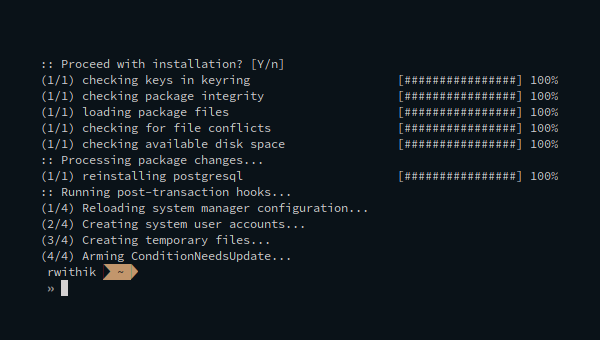
\includegraphics[width=\linewidth]{../Images/Installation/2.png}\newline
\item You can switch to the PostgreSQL user by executing the following command:
\begin{minted}{bash}
$ sudo -iu postgres
\end{minted}
\end{enumerate}

\subsection{Initial Configuration}

\begin{enumerate}
\item A database cluster must be initialized before \mintinline{psql}{postgres} can be used. Execute the following command as the postgres user:
\begin{verbatim}
$ initdb -D /var/lib/postgres/data
\end{verbatim}
where -D option gives the location of the database cluster.
Other optional arguments include:
\begin{verbatim}
--locale=locale, where locale is to be chosen amongst the
system's available locales
-E encoding for the encoding (which must match the chosen locale);
\end{verbatim}
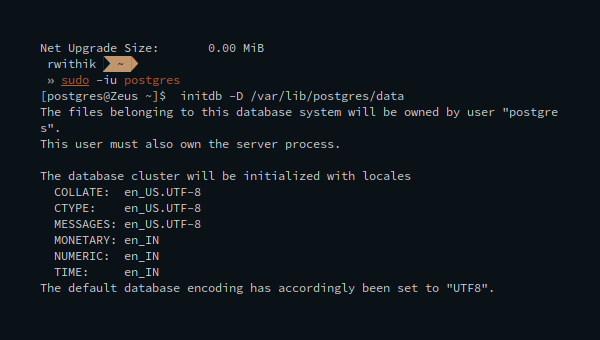
\includegraphics[width=\linewidth]{../Images/Installation/3.png}\newline
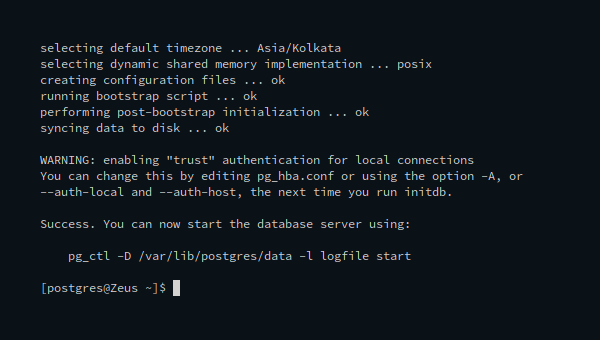
\includegraphics[width=\linewidth]{../Images/Installation/4.png}\newline
\item Start and enable \verb-postgresql.service-.
\begin{verbatim}
$ sudo systemctl start postgesql.service
$ sudo systemtcl enable postgresql.service
\end{verbatim}
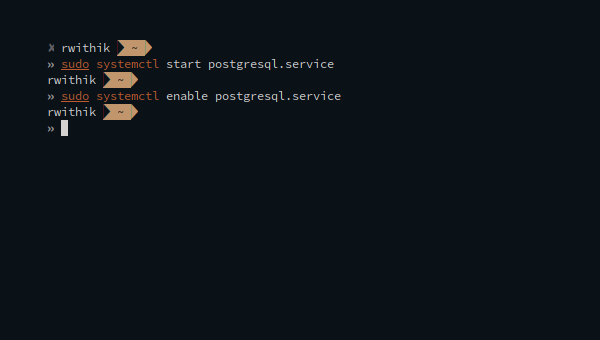
\includegraphics[width=\linewidth]{../Images/Installation/5.png}\newline
\item Create a new database user. Execute this command as the \verb-postgres- user:
\begin{verbatim}
$ createuser --interactive
\end{verbatim}
\item Create a new database. Run this command as the regular user:
\begin{verbatim}
$ createdb myDatabaseName
\end{verbatim}
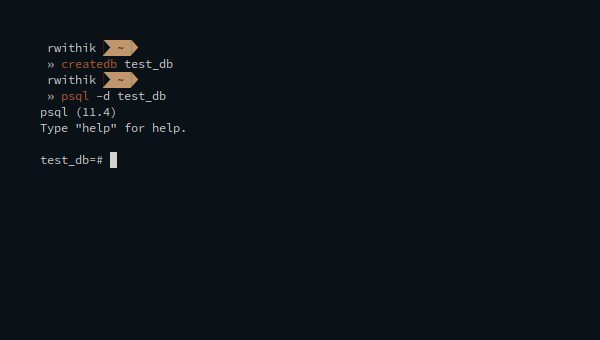
\includegraphics[width=\linewidth]{../Images/Installation/6.png}\newline

\end{enumerate}

\section{Result}
POSTGRESQL 11.5 was installed on Manjaro Linux and the configuration was done successfully.